\documentclass[../../../../main.tex]{subfiles}
\begin{document}

\begin{flushright}
\footnotesize\textit{【自動文字起こし・要確認】}
\end{flushright}

[解] (1) $PQ = x, QS = y, QR = z$ (いずれも正) とおくと、
ピタゴラスから
\[ \begin{cases} a^2 = x^2 + y^2 \\ a^2 = x^2 + z^2 \end{cases} \cdots \text{①} \]
だから、四面体の体積$V$として
\[ V = \frac{1}{6}xyz = \frac{1}{6}x(a^2-x^2) \quad (\because \text{①}) \quad (0 < x < a) \]
\[ \frac{d}{dx}V = \frac{1}{6}(a^2-3x^2) \]
から下表をえる

\begin{center}
\begin{tabular}{|c|c|c|c|c|}
\hline
$x$ & $0$ & $\cdots$ & $\frac{\sqrt{3}}{3}a$ & $a$ \\ \hline
$V'$ & & $+$ & $0$ & $-$ \\ \hline
$V$ & & $\nearrow$ & & $\searrow$ \\ \hline
\end{tabular}
\end{center}

よって、$\max V$ は $x = \frac{\sqrt{3}}{3}a$ のときの $\frac{\sqrt{3}}{27}a^3$

\begin{center}
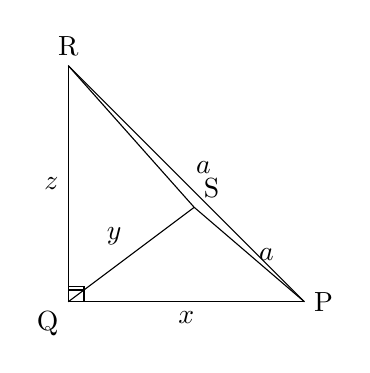
\begin{tikzpicture}[scale=2]
\coordinate (Q) at (0,0);
\coordinate (P) at (1.5,0);
\coordinate (R) at (0,1.5);
\coordinate (S) at (0.8,0.6);

\draw (Q) -- (P) node[midway, below] {$x$};
\draw (Q) -- (R) node[midway, left] {$z$};
\draw (Q) -- (S) node[midway, above left] {$y$};
\draw (P) -- (S) node[midway, right] {$a$};
\draw (P) -- (R) node[midway, above right] {$a$};
\draw (S) -- (R);

\node[below left] at (Q) {Q};
\node[right] at (P) {P};
\node[above] at (R) {R};
\node[above right] at (S) {S};

\draw (0.1,0) -- (0.1,0.1) -- (0,0.1);
\draw (0.1,0) -- (0.1,0.075) -- (0,0.075);
\end{tikzpicture}
\end{center}

(2) $AC$の中点$M$とする。対称性から $AC \perp MB, AC \perp DM$ であり、四面体$ABCD$の体積$V$、四面体$ABDM$の体積$V'$として
\[ V = 2V' \cdots \text{②} \]
である。面$\triangle ABM$を固定して $\angle BMD = \alpha \ (0 < \alpha < \pi)$ をうごかすと底面積を考えて$V'$は
$\alpha = \frac{\pi}{2}$ で$\max$である。この時の体積は(1)から $\frac{\sqrt{3}}{27}a^3$ だから ②に代入
\[ V = \frac{2\sqrt{3}}{27}a^3 \]

\begin{center}
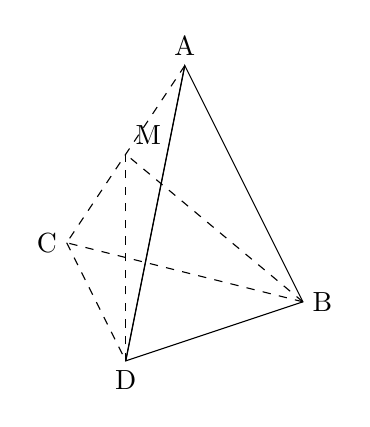
\begin{tikzpicture}[scale=1.5]
\coordinate (A) at (0,2);
\coordinate (B) at (1,0);
\coordinate (C) at (-1,0.5);
\coordinate (D) at (-0.5,-0.5);
\coordinate (M) at (-0.5, 1.25);

\draw (A) -- (B) -- (D) -- cycle;
\draw (A) -- (D);
\draw[dashed] (A) -- (C);
\draw[dashed] (B) -- (C);
\draw[dashed] (C) -- (D);
\draw[dashed] (B) -- (M);
\draw[dashed] (D) -- (M);

\node[above] at (A) {A};
\node[right] at (B) {B};
\node[left] at (C) {C};
\node[below] at (D) {D};
\node[above right] at (M) {M};
\end{tikzpicture}
\end{center}

\begin{center}
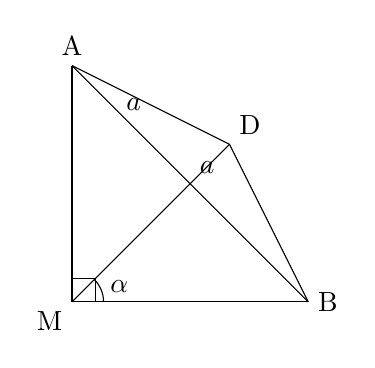
\begin{tikzpicture}[scale=2]
\coordinate (M) at (0,0);
\coordinate (A) at (0,1.5);
\coordinate (B) at (1.5,0);
\coordinate (D) at (1,1);

\draw (M) -- (A);
\draw (M) -- (B);
\draw (M) -- (D);
\draw (A) -- (B) node[midway, above right] {$a$};
\draw (A) -- (D) node[midway, left] {$a$};
\draw (B) -- (D);

\node[below left] at (M) {M};
\node[above] at (A) {A};
\node[right] at (B) {B};
\node[above right] at (D) {D};

\draw (0.2,0) arc (0:45:0.2);
\node at (0.3,0.1) {$\alpha$};
\draw (0,0.15) -- (0.15,0.15) -- (0.15,0);
\end{tikzpicture}
\end{center}

\end{document}
